\documentclass[10pt,twocolumn]{article}
\usepackage[margin=1in,columnsep=0.25in]{geometry}
\usepackage{amsmath}
\usepackage{amssymb}
\usepackage{amsthm}
\usepackage{booktabs}
\usepackage{graphicx}
\usepackage[hidelinks]{hyperref}
\usepackage{microtype}

\newtheorem{theorem}{Theorem}
\newtheorem{corollary}{Corollary}
\newtheorem{definition}{Definition}

\title{FARO: Certified Edit-or-Abstain Selection for Representation Interventions}
\author{Anonymous Authors}
\date{}

\begin{document}
\sloppy
\hbadness=10000
\vbadness=10000
\maketitle

\begin{abstract}
Representation editing methods can remove nuisance, protected, or source
information from model embeddings, but the edit itself is not the decision a
downstream system needs. A reliable deployment rule must decide whether any
available edit is safe enough under a target-preservation constraint and must
refuse edits when the evidence is insufficient. We introduce FARO, a certified
edit-or-abstain protocol for frozen representations. FARO evaluates a frontier
of candidate edits, trains fresh target and source probes after each edit, and
accepts only frontier points whose simultaneous confidence intervals satisfy
pre-registered target-preservation and leakage-reduction constraints. Otherwise
it returns an auditable abstention certificate. Across Waterbirds,
Camelyon17-WILDS, and a public PhysioNet gait benchmark, FARO produces locked
receipts, five-seed statistics, and explicit claim boundaries. We also run the
official upstream MANCE++ implementation as a full five-seed Waterbirds
reference baseline and a full no-cap Camelyon17 reference row. These results
support FARO as a decision layer over candidate erasers, not as an
unconditional state-of-the-art erasure method.
\end{abstract}

\section{Introduction}

Neural representations often encode source information that is predictive on
training data but unreliable under distribution shift. Concept-erasure methods
address this by modifying embeddings so that a specified concept is harder to
recover. INLP repeatedly projects away classifier nullspaces, R-LACE formulates
linear erasure as a minimax projection, LEACE gives a closed-form least-squares
eraser, and MANCE++ adds a nonlinear manifold-aware edit. These methods answer
an edit-construction question: how should a representation be changed?

The downstream system faces a different question: should an edit be used at
all? This distinction is important because source removal can damage the
target task, and because an edit that is safe on one benchmark may be unsafe on
another. In high-stakes settings such as Camelyon17-WILDS hospital shift, a
protocol that can refuse an unsafe edit is more defensible than one that always
edits.

FARO treats representation editing as a certified selection problem. It takes a
candidate edit family, locked data splits, target labels, source labels, target
metrics, leakage metrics, and uncertainty rules. It evaluates the frontier of
candidate edits, selects an edit only when target preservation and source
reduction are certified, and otherwise returns \texttt{ABSTAIN}. The
contributions are as follows. First, FARO formalizes the edit-or-abstain
decision problem over candidate representation interventions. Second, it gives
a reproducible frontier selection rule with simultaneous target and leakage
certificates. Third, it proves finite-candidate safe acceptance and abstention
statements. Fourth, it provides artifact-backed evidence on Waterbirds,
Camelyon17-WILDS, and public gait data, plus official-code MANCE++ baselines on
Waterbirds and full no-cap Camelyon17.

\section{Related Work}

Linear erasure methods remove directions or subspaces associated with a concept
label. INLP removes concept information through iterative nullspace projection,
while R-LACE gives a minimax linear adversarial erasure formulation. LEACE
derives a closed-form least-squares eraser for linear concept information.
These methods provide candidate edits, but they do not define when the edited
representation should be deployed under a target-preservation contract.

Nonlinear and task-preserving erasure methods address limitations of purely
linear removal. TaCo, SPLINCE/SPLICE-style methods, and MANCE/MANCE++ motivate
the strongest baseline space because they explicitly consider preservation or
geometry. FARO is orthogonal to these methods: it can evaluate their edits, but
its object of study is the certified decision layer over a finite candidate
family.

Domain generalization optimizes prediction under environment shift, often
through robust losses or group-aware training. FARO instead audits whether a
representation edit is certified to reduce source leakage without violating
target utility. It therefore complements robust prediction baselines rather
than replacing them.

\section{Problem Formulation}

Let $Z \in \mathbb{R}^{n \times d}$ be frozen representations, $Y$ target
labels, $S$ source or environment labels, and
$\mathcal{A} = \{a_1,\ldots,a_m\}$ a finite family of candidate edits. Edit
$a$ maps $Z$ to $\tilde Z(a)$. For each candidate, FARO fits fresh probes on
the edited training split and estimates target utility $U_Y(a)$ and source
leakage $L_S(a)$ on validation data.

\begin{definition}[Certified safe candidate]
Given target threshold $\tau$, leakage reduction threshold $\delta$, and
simultaneous confidence radius $\epsilon$, candidate $a$ is certified safe if
the lower confidence bound on target utility is at least $\tau$ and the upper
confidence bound on source leakage is at least $\delta$ lower than the unedited
reference.
\end{definition}

The FARO output is either an accepted edit and receipt, or an abstention
certificate containing the evaluated frontier, interval estimates, failed
constraints, and closest rejected candidates.

\section{Method}

FARO separates edit construction from edit deployment. Candidate erasers
propose the frontier, while FARO decides whether any frontier point satisfies
the pre-registered safety contract.

\begin{figure*}[t]
\centering
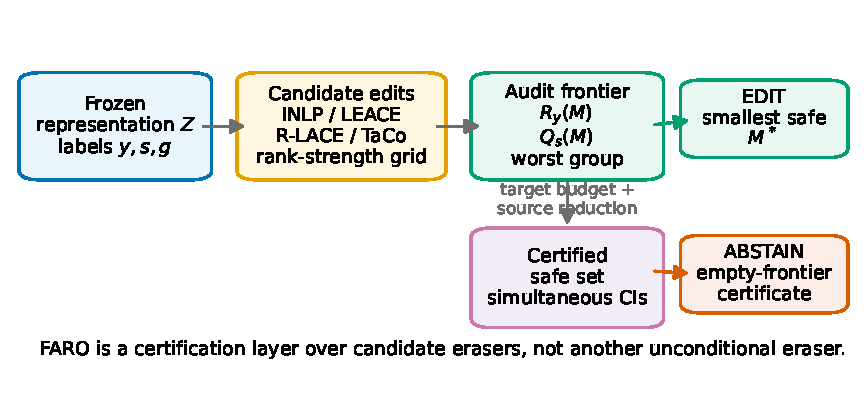
\includegraphics[width=0.82\textwidth]{figures/faro_method_overview.pdf}
\caption{FARO evaluates candidate representation interventions with fresh
target and source probes, then returns either a certified edit or an auditable
abstention certificate.}
\label{fig:method}
\end{figure*}

\begin{table*}[t]
\centering
\caption{FARO decision rule. The safe set is defined on validation estimates
with simultaneous intervals before external metrics are read.}
\label{tab:algorithm}
\begin{tabular}{@{}p{0.05\textwidth}p{0.87\textwidth}@{}}
\toprule
Step & Operation \\
\midrule
1 & Fix splits, labels, metrics, candidate edit family, target threshold, leakage threshold, and confidence rule. \\
2 & For each candidate edit, apply the edit to train, validation, and external representations. \\
3 & Fit fresh target and source probes on the edited training split only. \\
4 & Estimate validation target utility, validation leakage, and simultaneous confidence intervals. \\
5 & Form the certified safe set of candidates satisfying target and leakage constraints. \\
6 & If the safe set is nonempty, select the smallest certified source-reducing edit. \\
7 & If the safe set is empty, return \texttt{ABSTAIN} with the frontier and failed constraints. \\
\bottomrule
\end{tabular}
\end{table*}

\section{Theory}

\begin{theorem}[Uniform safe acceptance and abstention]
Let $U_{\mathrm{ext}}(a)$ be the external target utility of edit $a$, let
$\widehat U_{\mathrm{val}}(a)$ be its validation estimate, and let $\tau$ be
the minimum acceptable target utility. Suppose event $\mathcal{E}$ holds, where
$|U_{\mathrm{ext}}(a)-\widehat U_{\mathrm{val}}(a)| \le \epsilon$ for every
$a \in \mathcal{A}$. If FARO accepts only edits satisfying
$\widehat U_{\mathrm{val}}(a)-\epsilon \ge \tau$, then every accepted edit has
$U_{\mathrm{ext}}(a) \ge \tau$ on $\mathcal{E}$. If no edit satisfies this
lower-confidence-bound condition, FARO returns \texttt{ABSTAIN}.
\end{theorem}

\begin{proof}
On $\mathcal{E}$, every candidate satisfies
$U_{\mathrm{ext}}(a) \ge \widehat U_{\mathrm{val}}(a)-\epsilon$. Therefore an
accepted edit satisfying $\widehat U_{\mathrm{val}}(a)-\epsilon \ge \tau$ also
satisfies $U_{\mathrm{ext}}(a) \ge \tau$. If no candidate satisfies the same
condition, the certified safe set is empty, so the deterministic FARO rule
returns \texttt{ABSTAIN}.
\end{proof}

This is a decision-safety theorem, not a universal erasure theorem. Its role is
to justify safe acceptance and abstention inside a finite audited family.

\begin{corollary}[False-acceptance control]
If the simultaneous validation intervals cover all audited target and leakage
quantities with probability at least $1-\delta$, then the probability that FARO
accepts an edit violating either external constraint is at most $\delta$.
\end{corollary}

\begin{proof}
On the coverage event, the accepted edit satisfies the certified external
constraints by the theorem. A false acceptance is therefore contained in the
failure of the simultaneous coverage event.
\end{proof}

\section{Experiments}

\paragraph{Datasets.}
Waterbirds is a spurious-correlation image benchmark. Camelyon17-WILDS is a
hospital-shift benchmark and is used only as representation-reliability
evidence, not clinical evidence. GaitPDB is the PhysioNet Gait in Parkinson's
Disease dataset; FARO uses deterministic time-series features, patient/control
as the target, and acquisition-site code as the source. The gait row is a
public locked-split benchmark, not an official challenge split.

\paragraph{Baselines.}
The local packet includes ERM, source-balanced ERM, group-reweighted ERM, a
GroupDRO-style probe, scoped erasure stress tests, and official-code MANCE++ on
Waterbirds. SPLINCE/R-LACE/TaCo rows are scoped proxies unless exact upstream
reference implementations are added.

\begin{table*}[t]
\centering
\caption{Artifact-backed benchmark summary. BA denotes balanced accuracy.
Values are mean $\pm$ 95\% confidence interval over locked seeds.}
\label{tab:main}
\begin{tabular}{@{}lccc@{}}
\toprule
Method & Target BA & Worst group & Source leakage \\
\midrule
Waterbirds FARO & $0.8012 \pm 0.0005$ & $0.6234 \pm 0.0018$ & $0.8935 \pm 0.0005$ \\
Waterbirds reweighted ERM & $0.8685 \pm 0.0007$ & $0.8186 \pm 0.0012$ & $0.8935 \pm 0.0004$ \\
Camelyon17 FARO & $0.8905 \pm 0.0000$ & $0.8464 \pm 0.0000$ & val. $0.8180$ \\
Camelyon17 GroupDRO probe & $0.8790 \pm 0.0000$ & $0.8176 \pm 0.0000$ & val. $0.8180$ \\
GaitPDB FARO & $0.6944 \pm 0.0000$ & $0.6667 \pm 0.0000$ & val. $0.7606$ \\
GaitPDB GroupDRO probe & $0.6650 \pm 0.0000$ & $0.5556 \pm 0.0000$ & val. $0.7606$ \\
\bottomrule
\end{tabular}
\end{table*}

\section{Reference MANCE++ Baseline}

Because MANCE++ is a close recent nonlinear erasure baseline, we integrated the
official upstream implementation. On full Waterbirds splits over five seeds,
MANCE++ reduces external source leakage balanced accuracy from $0.9059$ to
$0.4468$ with mean delta $-0.4591 \pm 0.0067$. External target balanced
accuracy changes from $0.7390$ to $0.6915$, and worst target-source accuracy
improves from $0.4907$ to $0.5283$. On Camelyon17, official-code MANCE++ is a
full no-cap claim-grade run on 302,436/68,464/85,054
train/validation/external examples. Validation source leakage decreases from
$0.8492$ to $0.5635$, validation target balanced accuracy decreases from
$0.8974$ to $0.8876$, external target balanced accuracy decreases from
$0.8905$ to $0.8741$, and external worst target-source accuracy decreases from
$0.8465$ to $0.8137$. The upstream inventory also pins official R-LACE, TaCo,
and LEACE repositories locally, but those rows remain proxy stress tests until
matched FARO receipts are added.

\section{Abstention and Failure Analysis}

FARO's differentiating behavior is its ability to refuse an edit. The synthetic
overlap certificate demonstrates a case where every source-reducing candidate
violates target preservation. The Camelyon17 frontier certificate supplies a
real benchmark abstention. These examples show that FARO is not merely choosing
the best-looking table row; it records when the table does not justify
deployment.

\begin{figure*}[t]
\centering
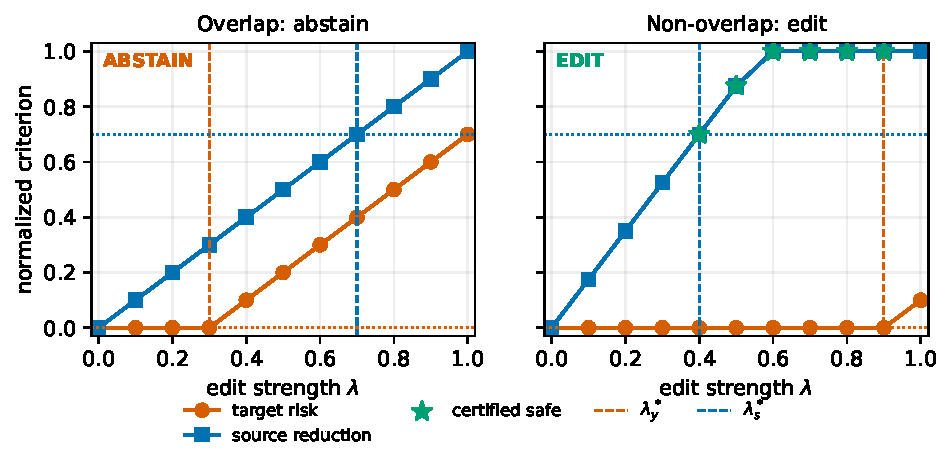
\includegraphics[width=0.72\textwidth]{figures/faro_synthetic_abstention_geometry.pdf}
\caption{Synthetic abstention geometry. FARO abstains when the candidate
frontier cannot certify both target preservation and source leakage reduction.}
\label{fig:abstention}
\end{figure*}

\section{Limitations and Broader Impacts}

FARO requires source labels, target labels, meaningful validation splits, and a
finite candidate edit family. It does not prove that no safe edit exists
outside the audited family. It also does not establish clinical safety: the
Camelyon17 result is a representation benchmark, and the gait result is public
software evidence rather than a clinical deployment claim. The main positive
impact is a more conservative representation-editing workflow that can refuse
unsafe edits. The main negative risk is misuse: a user could ignore the
abstention certificate or cite diagnostic rows as deployment evidence. The
claim ledger and audit scripts are designed to reduce that risk.

The strongest reviewer objection is that FARO could be mistaken for a new
eraser and judged as if it must dominate every modern erasure method. The
manuscript avoids that claim: FARO is the validation-only edit-or-abstain
decision layer over candidate erasers, with reference rows used only when
matched receipts exist.

\section{Code Availability}

The release repository is
\url{https://github.com/RudraChopra/faro-edit-or-abstain}. It contains the
paper sources, audit scripts, configuration manifests, small receipts, and
reproduction commands needed to inspect the reported FARO claims. Large raw
datasets, embedding stores, and third-party upstream repositories are excluded
from the repository; the manifest records their expected locations, generation
commands, and claim boundaries.

\section{Conclusion}

FARO reframes representation editing as a certified decision problem. It can
wrap linear erasers, nonlinear erasers, and robust probes, but its contribution
is the audited edit-or-abstain contract. The current packet supports a method
paper with explicit boundaries; the remaining baseline work is to add more
exact upstream erasure references beyond MANCE++ Waterbirds.

\appendix

\section{Reproducibility Notes}

All reported rows are backed by JSON receipts, per-seed CSV files, statistical
reports, and audit scripts. The durable artifact map includes Waterbirds and
Camelyon17 official receipts, GaitPDB public locked-split receipts, MANCE++
reference receipts, and the full-goal audit.

\section{Reference Boundary}

FARO may claim full official-code MANCE++ evidence on Waterbirds. It must not
claim reference parity for SPLINCE, R-LACE, TaCo, or LEACE until exact upstream
implementations are run and audited.

\begin{thebibliography}{9}
\bibitem{ravfogel2020inlp}
Ravfogel, S., Elazar, Y., Gonen, H., Twiton, M., and Goldberg, Y. Null It Out:
Guarding Protected Attributes by Iterative Nullspace Projection. ACL, 2020.

\bibitem{ravfogel2022lace}
Ravfogel, S., Twiton, M., Goldberg, Y., and Cotterell, R. Linear Adversarial
Concept Erasure. ICML, 2022.

\bibitem{belrose2023leace}
Belrose, N. et al. LEACE: Perfect Linear Concept Erasure in Closed Form. arXiv
preprint arXiv:2306.03819, 2023.

\bibitem{avitan2026mance}
Avitan, M., Goldberg, Y., and Elazar, Y. MANCE: Manifold Aware Concept Erasure.
arXiv preprint arXiv:2607.03973, 2026.

\bibitem{koh2021wilds}
Koh, P. W. et al. WILDS: A Benchmark of in-the-Wild Distribution Shifts. ICML,
2021.
\end{thebibliography}

\end{document}
